\newpage
\section{Proofs}
\subsection{Proof of Lemma 1}

\begin{proof}[Proof of Lemma 1]
    The marginal likelihood $p(y|k,\xi)$ is given by
    \begin{equation*}
        p(y|k,\xi)=p(y|Z) = \int_{(0,\infty)} \int_{\mathbb{R}^\nu} p(y|Z,\beta,\sigma) \pi(\beta|Z,\sigma)\pi(\sigma) d\beta d\sigma.
    \end{equation*}
    According to the specified priors, we have
    \begin{equation*}
        \begin{split}
            p(y|Z,\beta,\sigma) = \frac{1}{(2\pi\sigma^2)^{m/2}}\exp\{-\frac{1}{2\sigma^2}(y-Z\beta)^\top(y-Z\beta)\},\\
            \pi(\beta|Z,\sigma) = \frac{1}{(2\pi m \sigma^2)^{\nu/2}}|Z^\top Z|^{1/2}\exp \{ -\frac{1}{2m\sigma^2} \beta^\top Z^\top Z\beta\}.
        \end{split}
    \end{equation*}
    Then the Fubini Thm implies that,
    \begin{equation*}
        p(y|k,\xi) = \int_0^\infty \frac{1}{(2\pi \sigma^2)^{m/2} (m+1)^{\nu/2} } \exp \{-\frac{1}{2\sigma^2} a_{k,\xi}\} \pi(\sigma) d\sigma,
    \end{equation*}
    where $a_{k,\xi}=y^\top (I_m-\frac{m}{m+1}Z(Z^\top Z)^{-1}Z^\top)y$. With change of variables $w = \sigma / \sqrt{a_{k,\xi}}$, we have $p(y|k,\xi)\propto (m+1)^{-\nu/2}a_{k,\xi}^{-m/2}$. It follows from $\pi(k,\xi)\propto \tau(\mathcal{M}_k)^{-\gamma}$ that $p(k,\xi|y)\propto (m+1)^{-\nu/2}a_{k,\xi}^{-m/2}\tau(\mathcal{M}_k)^{-\gamma}$.
\end{proof}

\subsection{Proof of Lemma 3}

\begin{proof}[Proof of Lemma 3]
    According to (9),
    \begin{equation*}
        \alpha(k',\xi'|k,\xi) = \min \left\{1,~ \frac{p(k',\xi'|y)q(k,\xi|k',\xi')}{p(k,\xi|y)q(k',\xi'|k,\xi)}\right\}.
    \end{equation*}
    Notably, $\pi(k,\xi)q(k',\xi'|k,\xi)=\pi(k',\xi')q(k,\xi|k',\xi')$ under the priors and proposals. Then we have $\alpha(k',\xi'|k,\xi) = \min\{1,~ p(y|k',\xi')/p(y|k,\xi)\}$. Thus (6) implies this lemma. For the EBIC approximation, we substitute $\hat{p}$ for the corresponding $p$.
\end{proof}

\section{Additional simulation}

We conduct EBARS in the curve spline regression $(d=1,p=3)$ and the surface spline regression $(d=2,p=3)$. The performance is compared with BARS of \citet{10.1093/biomet/88.4.1055}, smoothing splines (SS) of \citet{green1994nonparametric} and thin plate splines (TPS) of \citet{10.1111/1467-9868.00374}. We calculate the predictive mean squared errors (MSE) for evaluation. Simulations show that the proposed method contributes to accurate predictions of all scenarios.

\subsection{Curve spline regression}

%We conduct EBARS in curve spline regression and compare its prediction performance with BARS method \citep{10.1093/biomet/88.4.1055} and smoothing spline (SS) method \citep{wahba1990spline,green1994nonparametric}. 
The curves and data samples involved are illustrated in the first column of Figure \ref{fig:curve}. It can be seen that data are generated from $4$ different smoothness functions, denoted as Cases $1.1-1.4$ respectively. Cases $1.1$ and $1.2$ are continuous, whereas Cases $1.3$ and $1.4$ are discontinuous with one or multiple breakpoints. The outcome noise is Gaussian with standard deviation $2$, $2$, $4$, $1$. We compare the prediction performance with BARS and SS in curve fitting. To demonstrate the effect of $\gamma$ in EBIC, we implement $3$ versions of EBARS with $\gamma=1,0.5,0$. All methods are evaluated under sample sizes $m=200,500$ and the experiment is repeated $50$ times in each setting.

\begin{figure}
    \centering
    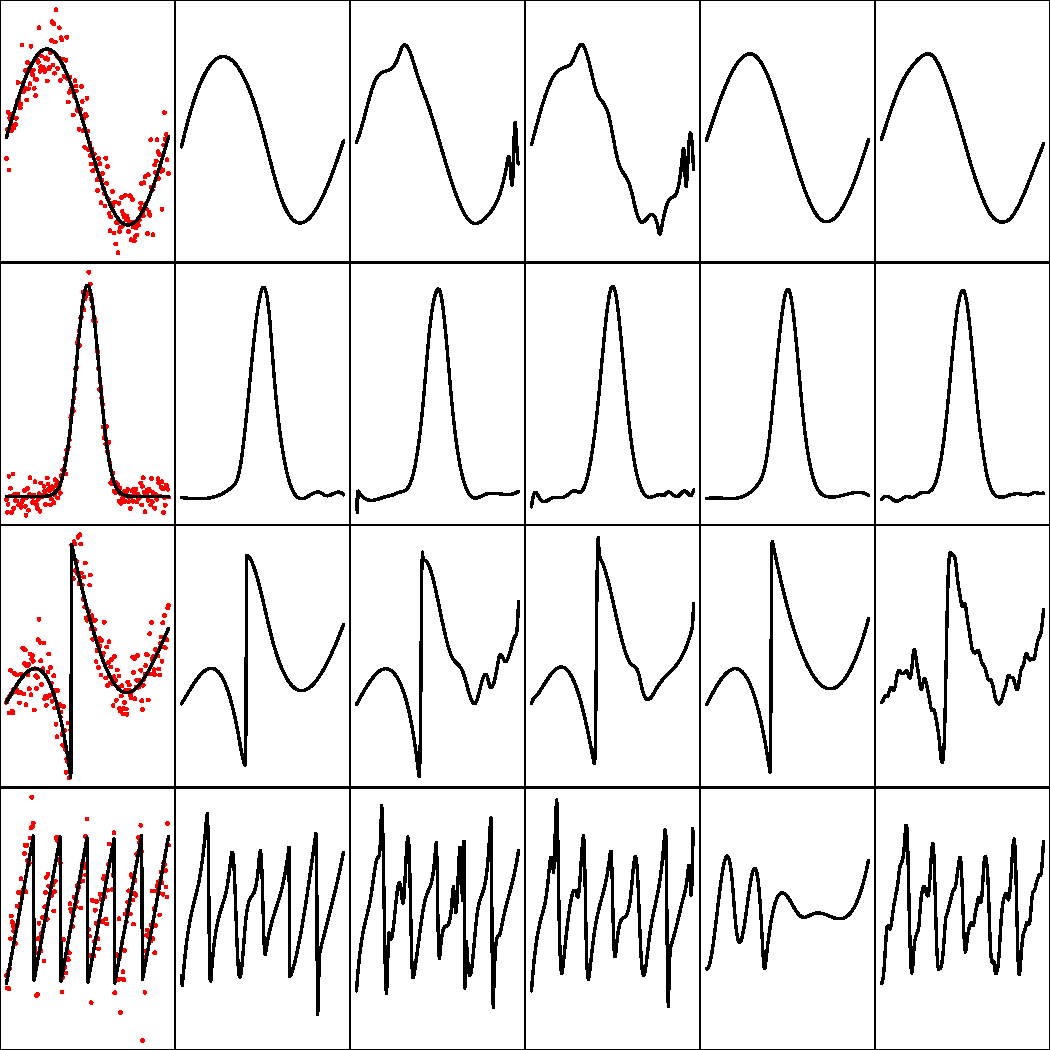
\includegraphics[width=0.85\textwidth]{Experiments/plots/curve_regression.pdf}
    \caption{Curve spline regression. It corresponds to the prediction results with $m=200$ in Cases $1.1-1.4$. From left to right, columns are respectively the ground truth with red observed points, prediction by EBARS with $\gamma=1,0.5,0$, prediction by BARS and prediction by smoothing splines.}
    \label{fig:curve}
\end{figure}

The mean squared errors are summarized in Table \ref{tab:curve}. To remove the effect of outliers, we drop out points with errors in the top or bottom $2.5\%$ to calculate censored MSE on test data. In EBARS, low $\gamma$ causes the model overfitting problem. It is clear that MSE rises up gradually as $\gamma$ decreases, especially in Case $1.3$. The behaviour is visualized in columns $2-4$ of Figure \ref{fig:curve}. This phenomenon is consistent with the theory. According to EBIC, the prior probability of the model space with $k$ knots satisfies $\pi(\mathcal{M}_k)\propto \tau(\mathcal{M}_k)^{1-\gamma}$. As $k<<n$ in practice, $\tau(\mathcal{M}_k)$ will grow with increasing number of knots. Consequently, the lower $\gamma$ means the higher $\pi(\mathcal{M}_k)$ for large $k$. Thereby more knots will be selected into the model, leading to overfitting in the end.

In this example, $\gamma=1$ gives the best performance among EBARS. Furthermore, BARS achieves similar results to EBARS $\gamma=1$ if the true knot number is relatively small, illustrated as in Cases $1.1-1.3$. However, when the required knot number is really large, BARS fails to work completely and attains a terrible MSE. See the $(4,5)$ panel of Figure \ref{fig:curve} for a graphical explanation. Besides, the smoothing spline method has a severe overfitting problem in Case $1.3$, as shown in the $(3,6)$ panel of Figure \ref{fig:curve}. This indicates that splines with many misplaced knots are inferior to adaptive knot splines in discontinuous cases.

\begin{table}
\caption{MSE on test data of five methods in Cases $1.1-1.4$}
\label{tab:curve}
\centering
\begin{tabular}{cccccccc}
\toprule
       Methods     &   $m$  & Case 1.1     & Case 1.2     & Case 1.3     & Case 1.4     \\ \midrule                               
                 
EBARS $\gamma=1$      & \multirow{5}{*}{$200$}     & 0.181(0.124) & 0.332(0.118) & 0.828(0.529) & 0.370(0.366)  \\
EBARS   $\gamma=0.5$  &       & 0.230(0.136)  & 0.389(0.184) & 1.412(0.783) & 0.368(0.150)  \\
EBARS   $\gamma=0$    &     & 0.341(0.229) & 0.464(0.201) & 1.960(0.985)  & 0.418(0.155) \\
BARS       &      & 0.178(0.150)  & 0.368(0.139) & 0.731(0.403) & 3.003(0.504) \\
SS &  & 0.137(0.088) & 0.329(0.132) & 3.772(1.687) & 0.443(0.155) \\
\midrule
EBARS $\gamma=1$     & \multirow{5}{*}{$500$}     & 0.068(0.033) & 0.147(0.061) & 0.361(0.168) & 0.079(0.033) \\
EBARS     $\gamma=0.5$   &    & 0.082(0.039) & 0.156(0.059) & 0.536(0.215) & 0.112(0.034) \\
EBARS    $\gamma=0$   &     & 0.170(0.073)  & 0.231(0.083) & 1.053(0.410)  & 0.144(0.042) \\
BARS        &     & 0.071(0.032) & 0.160(0.054)  & 0.317(0.140)  & 0.364(0.615) \\
SS & & 0.053(0.026) & 0.139(0.041) & 1.914(0.418) & 0.229(0.066) \\
\bottomrule
\end{tabular}
\end{table}
\subsection{Surface spline regression}

%We utilize tensor product splines to construct EBARS in bivariate spline regression and compare the performance with the BARS method and the thin plate spline (TPS) method of \citet{10.1111/1467-9868.00374}.
We compare the performance with BARS and TPS in the surface fitting.
%TPS is a popular spline-based approach for regression with multidimensional covariates.
The data is generated from four surfaces, denoted as Cases 2.1-2.4. Specifically, Cases 2.1 and 2.2 are smooth, whereas Cases 2.3 and 2.4 are discontinuous. Besides, Case 2.3 is with one jumping point in $x_1$ and Case 2.4 is with two jumping points in $x_1$ and $x_2$ separately. The outcome noise is Gaussian with standard deviation $1,1.5,2,2$. To remove outliers in discontinuous cases, we calculate MSE on test data without the upper or lower $2.5\%$ error. All methods are evaluated under sample sizes $m=500,1000$ and each experiment is repeated $20$ times.

\iffalse
\begin{figure}
    \centering
    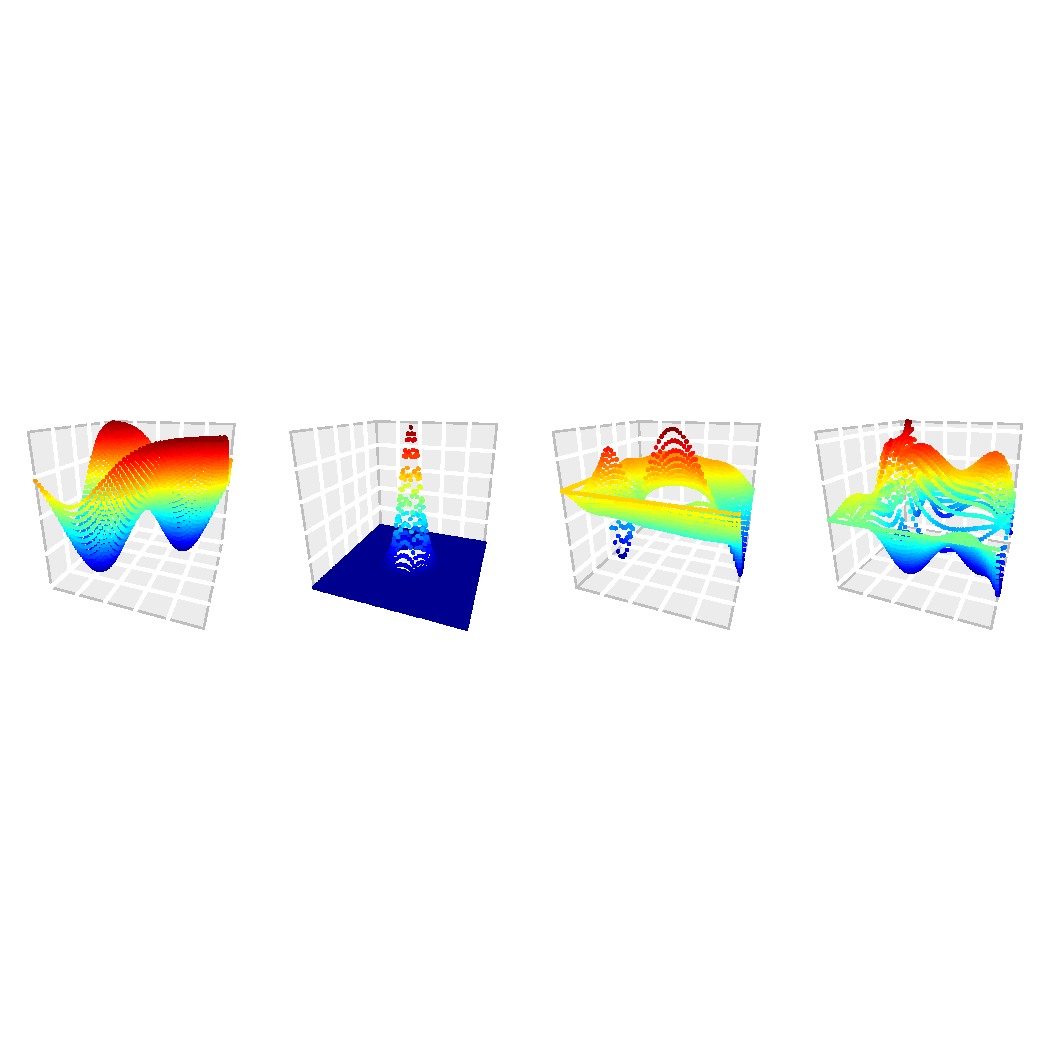
\includegraphics[width=1\textwidth]{Experiments/plots/crop_surface_truth.pdf}
    \caption{The ground truth in surface spline regression for Cases $2.1-2.4$. Cases 2.1 and 2.2 are continuous, whereas Cases 2.3 and 2.4 are discontinuous.}
    \label{fig:surface_truth}
\end{figure}
\fi

The mean squared errors are summarized in Table \ref{tab:surface}. Three EBARS versions with $\gamma=1,0.5,0$ are implemented to demonstrate the effect of $\gamma$. In Cases 2.1 and 2.2, the performance of all five methods is satisfactory and MSE of TPS is roughly the smallest. This indicates that five spline approaches do well in fitting smooth surfaces. However, when the surface is discontinuous, the prediction performance of TPS is worse than free knot splines. For example, the MSE of TPS are much larger than that of EBARS and BARS in Cases 2.3 and 2.4. BARS achieves close results to EBARS except for Case 2.4. As $k$ has to be large enough to fit Case 2.4, the performance of BARS is limited owing to the poor property of BIC in high dimension. Besides, EBARS performs slightly better with low $\gamma$ than with high $\gamma$ even in smooth cases, different from curve regression. It seems that surface regression is more likely to be underfitting rather than overfitting.

\begin{table}
\caption{MSE on test data of five methods in Cases $2.1-2.4$}
\label{tab:surface}
\centering
\begin{tabular}{cccccc}
\toprule
Methods & m                     & Case 2.1     & Case 2.2     & Case 2.3     & Case 2.4     \\
\midrule
EBARS $\gamma=1$   & \multirow{5}{*}{500}  & 0.163(0.044) & 0.624(0.107) & 0.664(0.216) & 1.133(0.443) \\
EBARS $\gamma=0.5$  &                       & 0.148(0.038) & 0.616(0.111) & 0.597(0.192) & 1.101(0.287) \\
EBARS  $\gamma=0$ &                       & 0.138(0.042) & 0.609(0.089) & 0.568(0.136) & 1.076(0.269) \\
BARS    &                       & 0.169(0.050) & 0.671(0.160) & 0.660(0.199) & 1.968(0.485) \\
TPS     &                       & 0.102(0.031) & 0.587(0.092) & 1.958(0.625) & 2.324(0.466) \\
\midrule
EBARS $\gamma=1$  & \multirow{5}{*}{1000} & 0.064(0.011) & 0.355(0.051) & 0.230(0.061) & 0.331(0.077) \\
EBARS $\gamma=0.5$  &                       & 0.066(0.016) & 0.326(0.056) & 0.222(0.053) & 0.343(0.078) \\
EBARS $\gamma=0$  &                       & 0.065(0.014) & 0.306(0.058) & 0.242(0.067) & 0.336(0.058) \\
BARS    &                       & 0.107(0.027) & 0.416(0.094) & 0.313(0.074) & 1.020(0.510) \\
TPS     &                       & 0.057(0.015) & 0.319(0.032) & 1.205(0.215) & 1.379(0.214) \\
\bottomrule
\end{tabular}
\end{table}

To graphically illustrate the difference in surface spline regression, we visualize the prediction results with $m=1000$ by contour maps in Figure \ref{fig:surface}. Initially, the fitted contours approximately overlap with the ground truth in Cases 2.1 and 2.2, see the top $2$ rows. We can see from the $(3,6)$ and $(4,6)$ panels that TPS fails to estimate the jump discontinuity in Cases 2.3 and 2.4. Actually, the fitted surfaces by TPS are always smooth regardless of the smoothness of true models. BARS obtains a nice performance in Cases 2.1-2.3, but is trapped in Case 2.4 when the required $k$ is enormous. Conversely, Columns $2-4$  of Figure \ref{fig:surface} show that our EBARS makes precise predictions in all cases successfully.

\begin{figure}
    \centering
    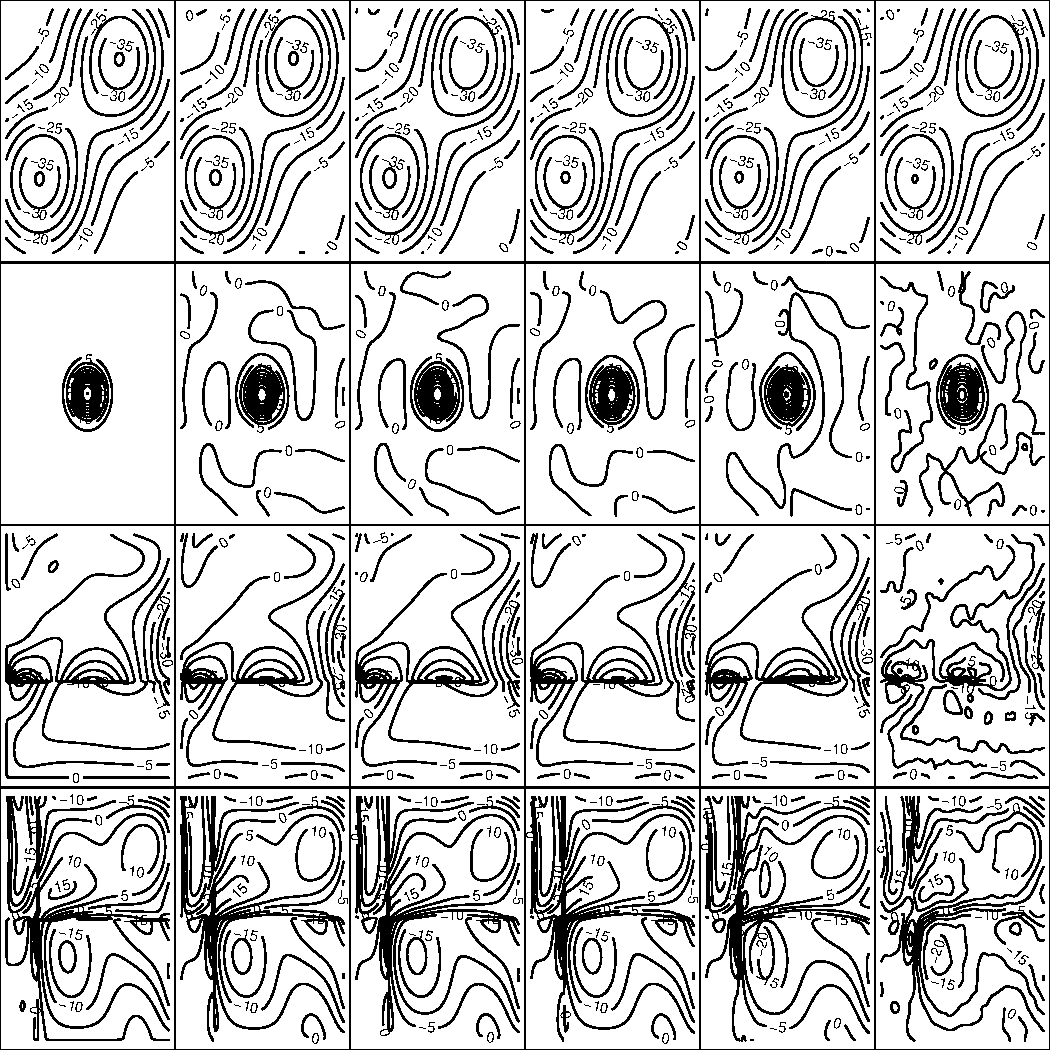
\includegraphics[width=0.85\textwidth]{Experiments/plots/surface_regression.pdf}
    \caption{Surface spline regression. It illustrates the prediction results with $m=1000$ in Cases $2.1-2.4$ by contours. From left to right, columns are respectively the ground truth, prediction by EBARS with $\gamma=1,0.5,0$, prediction by BARS and prediction by TPS.}
    \label{fig:surface}
\end{figure}
